\chapter{Thermal conductivity and the Earth's interior} % Main chapter title

\label{Chapter1} % Change X to a consecutive number; for referencing this chapter elsewhere, use \ref{ChapterX}

%-----------------------------------------------------------------------------------------------------------



%-----------------------------------------------------------
\section{Introduction to the problem}
%-----------------------------------------------------------

The nature of heat transport within a substance is controlled by its \tc. This influences the thermal evolution and heat budget of the Earth, but is poorly constrained across relevant conditions. Experiments can measure the conductivity of material, but not at the high pressure/temperature conditions found in the deep Earth. Computer simulations allow materials and their conductivities to be modelled on an atomic-scale, but care must be taken to achieve accurate results. This involves setting up the material to faithfully replicate its expected real-world counterpart, and choosing a simulation method which includes realistic atomic interactions. In this chapter, I will introduce thermal conductivity and the deep earth, considering the effects of the former on the latter.

%---------------------------------------
\subsection{Man-made applications with \tc}
%---------------------------------------
Knowledge of the thermal conductivity of solids is key for a wide range of technological applications, in addition to developing our understanding of natural systems. Conductivity determines whether a material is a conductor or insulator of heat, both of which have many uses, technological or otherwise. Oven gloves introduce an insulating, low conductivity layer between our hands and a hot object which would otherwise cause injury. Vacuum flasks utilise a low conductivity construction to keep liquids hot, houses have wall insulation to keep the heat in. While a saucepan may have an insulating rubber handle, it may also have a conductive copper base, allowing it to heat up quickly with an even temperature distribution.

Heat exchangers are found in many systems, where one substance is used to cool or heat another. While the heat transfer is affected by the thermal conductivity of the media in question, the material that seperates the two must have high conductivity for the system to be efficient. Domestic examples include central heating system, fridges, and cars. Industrial examples include solar water heating, and power plants, from geothermal to nuclear.

Thermoelectric materials convert waste heat into electricity, thereby improving the efficiency of domestic, automotive, and industrial processes. They are proposed to increase the sustainability of our current electricity base, but suitable materials must have a low thermal conductivity \citep{Snyder2008}.

%---------------------------------------
\subsection{Conductivity in the Earth}
%---------------------------------------

Within the lower mantle, thermal conductivity influences the rate at which heat is transferred from core cooling towards the surface, and more importantly the mechanisms by which it does so \citep{Lay2008}. High thermal conductivity systems will preferentially transport heat by conduction. Systems will convect (ADVECT?) where there is too much heat to be transpoted by conduction alone (i.e. low conductivity conditions).

Observations of plume structures and cyclic subduction patterns \citep[see][]{Garnero2008} suggest convective behaviour in the lower mantle. Thermal conductivity is poorly constrained in this region, obtaining a comprehensive depth profile is not a trivial task. Additional difficulties are pressure, temperature, and compositional dependences, including isotopic variation \citep{Tang2010,Dalton2013,Tang2014} and inclusion of impurities \citep{Manthilake2011,Ammann2014,Ohta2014}.

%---------------------------------------
\subsection{AIMS / WHAT DO I DO THAT IS DIFFERENT TO OTHERS}
%---------------------------------------

The aim of the work presented in this thesis is to model \tcs at the core mantle boundary (CMB). I will running simulations at high pressure and varying temperatures, considering the effects of composition across an entire solid solution. 

By parameterising the temperature and compositional-dependence, \tcs can be determined as a function of both at any condition. This is of particular use to LEMA because of REASONS. 

In order to perform this parameterisation, I will need to explore the equations that describe these dependencies, adapting them where necessary to compliment my result set.

Working on the atomic-scale, compositional variations are more important than in a sample of bulk material. A relatively low amount of possible sites for impurities to be placed means clumping is possible, and must be considered when randomly substituting atoms.

Fundamental characteristics of heat transport in atomic systems mean that the size of the system / number of atoms affect the magnitude of the conductivity result. Measures exist to quantify these effects, but simulations may yield incorrect results if system size is not considered. I will look into this to validate my calculated results, but also to offer analysis of these finite size effects (FSE) for atomic simulations in general.





%-----------------------------------------------------------
\section{Defining \tc}
%-----------------------------------------------------------
\label{sec:defining_tc}

Thermal conductivity is a material property, indicative of the ease with which heat is transferred through conduction. For known substances thermal conductivity spans about six orders of magnitude, from silica aerogels with 0.005~\wmks \citep{Lee1995} to graphene with 5000~\wmks \citep{Balandin2008}.

The transfer of thermal energy can occur between an object and its surroundings, two bodies brought into contact, or along a temperature gradient within an object. The possible mechanisms by which this can occur are conduction, convection, and radiation. Conduction is the transfer of heat by atomic vibrations and electron transport in metallic substances (such as in the outer core). Convection is the motion of thermal energy via a moving medium, generally in liquids and gases (but expected in the mantle). Density differences are the driving force for convection, due to the volume change associated with thermal expansion. Radiation refers to the transport of heat by electromagnetic radiation in the form of photons.

I am primarily concerned with the atomic vibrations of lattice conduction through the lower mantle, and secondly the convective behaviour therein. Mantle minerals are expected to be insulators, meaning there is no contribution from electron transport. The radiative component of thermal conductivity in the mantle is thought to be small \citep{Goncharov2008}, and will not be determined as part of this work. In the event that radiation contributes significantly to the effective thermal conductivity \citep{Keppler2008}, it can simply be added to the lattice component.

Convection in them mantle is dependent on the \tc, and will occur if heat cannot be sufficiently transported by conductive processes. The value of the Rayleigh number describes the behaviour of heat flow in a fluid, relative to a critical value for the system. Many variables are required to determine the Rayleigh number, but most importantly here it is inversely proportional to \tc. If the calculated Rayleigh number is lower than the critcal value, conduction is the dominant process. When the Rayleigh number is greater, the ratio between it and the critcal value decribes the vigour and style of convection.

%---------------------------------------
\subsection{Mechanisms of heat transport}
%---------------------------------------

The transport of heat, rather than the transport of hot material, can be split into three components that contribute to the overall thermal conductivity of a material. These transport mechanisms can be explained on an atomic level, and in the case of this study within a crystal lattice. Atoms have translational symmetry within a crystal, the lattice can be thought of a regular, repeating pattern of atomic arrangement. 

Electrical thermal conductivity refers to the transport of heat via free electrons in a lattice structure. Radiative thermal conductivity is the transport of heat via photons, or packets of electromagnetic energy. Phonons are packets of vibrational energy, a quasiparticle used to describe atomic motions which contribute to lattice thermal conductivity.

!!! DIAGRAM OF A LATTICE ??? CRYSTALMAKER ???

%-------------------
\subsubsection{Electron}
%-------------------

Close parallels exist between thermal and electrical conduction. The conduction of thermal energy in metals is predominantly due to the motion and interaction of free electrons. Heat is transferred as electrons move and collide in the lattice. There is no net transport of electrons in order to maintain charge neutrality within the lattice. Lower mantle minerals are semiconductors, and thus electrical thermal conductivity is of little significance to this project.

%-------------------
\subsubsection{Photon}
%-------------------

Any body with a non-absolute zero temperature emits thermal radiation as light, or photons. Radiative thermal conductivity is determined by a material's optical absorptivity, which describes how heat is transferred by electromagnetic radiation within a material. On the atomic scale, charged particles vibrate and emit light. Energy is transferred from one particle to another when this light is scattered or absorbed. The transfer of heat by radiation is limited similarly to the transfer of visible light, with difficulty passing through opaque media. Unlike lattice conductivity at mantle conditions, radiative conductivity increases with temperature \citep{Hofmeister1999}. This relation has been used to assume thermal conductivity could be constant through the lower mantle if radiative processes are significant, where the lattice component decreases at the same rate the radiative increases \citep{Tang2014}.

%-------------------
\subsubsection{Phonon}
%-------------------

!!! DEBYE DIAGRAM

!!! OPTICAL VS. ACOUSTIC EXPLAIN !!!

The final way heat is conducted is by the vibration of atoms, where the velocity of an atom is proportional to its heat. As an atom vibrates, forces act on neighbouring atoms, inducing motion. Hot atoms in a closed system transfer energy to cold atoms in this way, until energy and temperature are both equilibrated. Considering a crystalline arrangement of atoms, there is long-range structure and well-defined bonds between atoms. Much like standing waves on a string, atoms can vibrate in-phase. These patterns of vibrations are called phonons, and can be differentiated by wavelength and the relative motions of atoms.

Similar to how photons have wave particle duality, phonons are known as quasiparticles. This is useful for explaining how phonons ``waves'' interact with structural discontinuities and in phonon-phonon collisions. As a particle, a phonon is a quantised packet of vibrational energy. Unlike electronic heat conduction, there is a net motion of phonon ``particles'' from hot to cold regions. 

A phonon's mean free path (MFP) is the distance it travels before scattering. The further the average phonon travels, the more efficient the heat transport and thus higher the thermal condutivity. A number of effects cause phonons to scatter: (1) collisions with other phonons in the lattice, (2) boundaries or defects in the material, and (3) impurities in the atomic structure. The MFP can be determined with Matthiesen's rule, 

!!! INSERT EQUATION HERE

where [VARIABLE DECLARATION]. All sources of scattering are considered, but the shortest path dominates the MFP. This is displayed in the equation, where the inverse of the smallest number contributes the most to the sum.






%---------------------------------------
\subsection{What affects it?}
%---------------------------------------

!!! ADD THE EQUATION WITH CV AND V! 



%-------------------
\subsubsection{Pressure}
%-------------------

Volume of the material decreases with increasing pressure, with increasing depth into the Earth. This tends to increase the bulk and shear moduli, causing the seismic wave velocity to increase. Referring back to ABOVE EQUATION, increasing pressure causes a conductivity increase.

%-------------------
\subsubsection{Temperature}
%-------------------

!!! ADD NICE FIGURE

The amount of phonon ``modes'' contributing to heat transport increases with the material's heat capacity, until the saturation of this parameter at the Debye temperature. \Tc is proportional to the amount of active modes, so also increases with temperature up to the Debye limit. After this point, phonon-phonon scattering begins to reduce conductivity, as the frequency of more energetic collisions increases. Conductivity change is inversely proporitional to temperature at this point, decreasing, and eventually saturating, to a minimum value. Bridgmanite is above its Debye temperature for all lower mantle conditions I will consider. I can safely assume its conductivity will decrease with rising temperature.

%-------------------
\subsubsection{Composition}
%-------------------

Considering a ``pure'' material, like \mgsios \bdg, the two sources of scattering are phonon-phonon, and phonon-boundary. Addition of impurities, such as in \mgfesios \pv, introduces phonon-impurity scattering and can reduce conductivity. The effect of impurities is less significant at high temperatures, when conductivity is already reduced by phonon-phonon sacttering. When the phonon-impurity path is much shorter than those of other scattering sources however, impurities can greatly reduce conductivity. Because of these relations, impurities will affect conductivity more higher in the mantle, with the effect reducing towards the CMB. The effect of impurities on thermal conductivity will be discussed extensively in CHAPTER FOUR.



%-----------------------------------------------------------
\section{Structure of the Earth}
%-----------------------------------------------------------
\label{sec:earth_structure}

\begin{figure}[h!]
  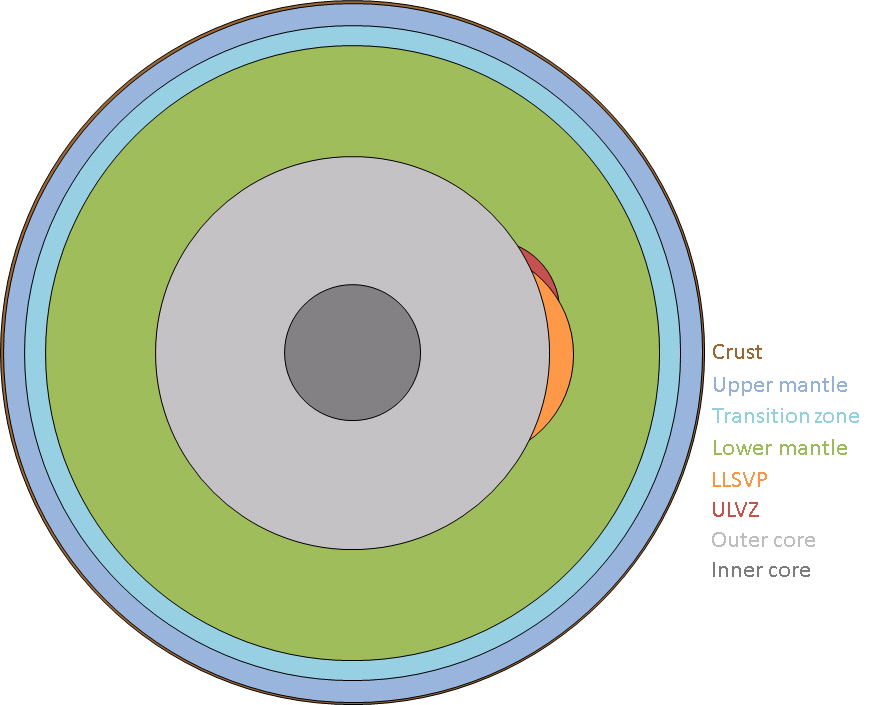
\includegraphics[width=\linewidth]{Figures/pp_earth_diagram.png}
  \caption[EARTH STRUCTURE DIAGRAM]{THE IDEA HERE IS FOR ME TO MAKE A FIGURE THAT INCLUDES ON THE MOST RELEVANT BITS OF THE EARTH, BASED OFF WHAT I MENTION IN FOLLOWING PARAGRAPHS. ADD SCALEBAR/DISTANCES? TEXT ON FIGURE? MARK CMB? MARK ATMOSPHERE/SURFACE?}
  \label{fig:earth_diagram}
\end{figure}

The average radius of the Earth is 6371~km, the properties of which change dramatically with depth to the centre. I will be focussed on the lower mantle, particularly the region close to the core (the core mantle boundary, CMB). Events in the lower mantle influence (and are influenced by) the upper mantle and lithosphere above, and the core below. Heat transport throughout the Earth is influenced by thermal conductivity, which in turn affects the dynamics of the system, the surface expression of this being plate tectonics. Heat flow also affects the core geodynamo, which produces the Earth's magnetic field. 

%---------------------------------------
\subsection{Lower mantle}
%---------------------------------------

The lower mantle encompasses the region after the mantle transition zone (660~km deep, $\sim$1900~K, $\sim$25~GPa) to the CMB (2900~km deep, $\sim$4000~K, 136~GPa). The composition of this region can be approximated as 75\% bridgmanite (MgSiO$_3$, magnesium silicate perovskite), 20\% periclase (MgO, magnesium oxide), and  5\% calcium silicate (CaSiO$_3$) perovskite \citep{Tronnes2009}. All of which are insulators and past their Debye temperatures at lower mantle conditions, with the potential for the inclusion of impurities such as iron and aluminium.

The exact nature of impurities is complicated to resolve, as there are a lot of variables. Iron comes in ferrous and ferric varieties, which can have varying electron spin states. The amount of iron is not partitioned evenly thoughout the mineral phases, periclase taking a larger proportion than bridgmanite for example. The nature of partitioning changes with physical conditions, where \ppvs may behave differently to \bdg.

A popular opinion is that bridgmanite is stable in the lower mantle until the bottom few 100~km, where it undergoes a pressure-driven phase change to post-perovskite \citep{Murakami2004,Oganov2004}. In places, close proximity to the CMB might transform post-perovskite back to perovskite structure due to the increased temperature. This ``double crossing'' of the bridgmanite stability range can be imaged seismically, where lens-like bands of post-perovskite are shown to pinch out laterally \citep{Lay2006}.

The lower mantle is not heterogeneous, with large-scale features around the CMB. Two large low shear velocity provinces (LLSVPs) can be found roughly underneath Africa and the Pacific. An associated feature is the ultra-low velocity zones (ULVZs), identified around the edges of LLSVPs. These can be observed seismically, but the reason they exist is unclear. It is suggested they are ``thermo-chemical features'', hotter and denser than the regular lower mantle. Increasing temperature and density tend to reduce seismic velocity, with increased density to offset the additional buoyancy from raised temperature. ``Thermo'' intuitively refers to the change in temperatures, while ``chemical'' changes are required to explain density increase. As a result, thermal conductivity will vary within these regions. Adding impurities such as iron would be a possible cause for density increase, such that the conductivity change should be quantified.

%---------------------------------------
\subsection{Lithosphere and upper mantle}
%---------------------------------------

The lithosphere (from 0~km depth) and upper mantle lie above the transition zone (to 660~km depth), which marks the top of the lower mantle. Although the chemistry of these regions is similar to that of the lower mantle, the physical conditions and mineral phases are different. Eruptive and subductive behaviour associated with plate tectonics is perhaps the most obvious consequence of mantle dynamics at the Earth's surface, and generally to humanity.

The ``rocky'' portion of the Earth (from the surface down to CMB) is largely some form of silicate mineral, often with magnesium and iron. The two main mineral transitions from the Earth's surface to the top of the lower mantle are pyroxene to garnet (40\%), and olivine through wadsleyite to ringwoodite \citep[60\%][]{Tronnes2009}. The olivine to wadsleyite change occurs at 410~km, marking the top of the mantle transition zone. Wadsleyite transitions to ringwoodite through this zone until 660~km, at which point it breaks down into lower mantle bridgmanite and ferropericlase.

%---------------------------------------
\subsection{Inner and outer core}
%---------------------------------------

The region beyond the CMB (starts at 2900~km depth) includes the core, comprised of its outer and inner sections. The liquid outer core extends to 5100~km depth, where the pressure-driven transition to solid inner core occurs. The composition of the core is dominated by iron, with various light elements suggested as possible alloying components.

Relative to the lower mantle, the outer core is a vigorously convecting system, and the core-side CMB can be considered to be an isothermal boundary. The main relevance to the lower mantle is the heat transfer across the CMB, the rate of which depends on the mantle conductivity and temperature. A second concern is that of chemical transfer between core and mantle, where iron from the core would be swapped various light mantle elements. Fe-content may increase in the lower mantle with CMB proximity, which in turn affects conductivity and the temperature profile for CMB heat flux.





%-----------------------------------------------------------
\section{Previous work - geophysics}
%-----------------------------------------------------------

%---------------------------------------
\subsection{STUFF THAT IS INFLUENCED BY CONDUCTIVITY}
%---------------------------------------
\label{sec:ch1:cond_in_earth}

Thermal conductivity in the deep Earth influences dynamic processes such as mantle convection and heat loss from the core \citep{Lay2008}. In this section I will discuss the prominent thermal conductivity-dependent processes.

%-------------------
\subsubsection{Mantle dynamics}
%-------------------

In the lower mantle \tcs changes with pressure, temperature, and composition, influencing features on a large scale. For example, \citet{Naliboff2006} used numerical models of mantle convection to show size and stability of convective plumes are sensitive to thermal conductivity above the core mantle boundary (CMB).

\citet{Dubuffet2000} investigated the effects of temperature and pressure-dependent \tcs on mantle convection, finding that depth-dependent \tcs encouraged heat transport via convective plumes. Compared to a constant conductivity model, vertical heat transfer was concentrated to these ``pipe-like'' structures, despite the horizontally-averaged heat flow for both systems being around the same value. Variable conductivity, even in one dimension, increased the spatial and temporal stability of convection. Plumes were thicker, had heads of larger surface area, and were hotter, compared to the uniform conductivity mantle model.

%-------------------
\subsubsection{Heat flow}
%-------------------

The most accessible estimate of the Earth's energy is the total heat flow at the surface, of which a value of $46\pm3$~TW is accepted as the upper bound. Sources of surface heat flow include; radiogenic heating ($20\pm3$~TW), mantle cooling (8--28~TW), and the conduction of heat across the CMB from core cooling \citep{Lay2008}. Conductive heat flow is constrained by thermal conductivity, a model of which is not available for all Earth conditions.

Better constraints on thermal conductivity are required to estimate CMB heat flow. This in turn would tell us more about the temperatures either side of the CMB, as well as the presence and nature of the lower mantle thermal boundary layer (TBL). Employing the most commonly used value for lower mantle conductivity, 10~\wmk~\citep{Lay2008}, heat flow across the CMB is expected to be 5--13~TW~\citep{Lay2008}. The value of 10~\wmks used by \citet{Lay2006} is an estimate of lowermost mantle \tc, based on extrapolation of a measurement at ambient conditions \citep{Osako1991}. Both higher and lower values have been proposed \citep[4--16~\wmk,][]{Manthilake2011}, illustrating how poorly constrained thermal conductivity is at CMB-relevant pressure/temperature conditions.

%-------------------
\subsubsection{Geomagnetism}
%-------------------

Using shear wave velocity as a proxy for CMB heat flow, \citet{Gubbins2007} showed that variations in mantle temperature gradients above the CMB can influence Earth's geodynamo. The present day magnetic field at the surface has four lobes, and these align above regions of fast shear wave velocity on the CMB. Ignoring compositional effects in the mantle, seismically-fast regions can be assumed to be cold. Considering Fourier's law (CITE), colder regions facilitate larger heat flows through steeper temperature gradients from the isothermal CMB.

\citet{Gubbins2007} recreate the geomagnetic observation of the aforementioned lobes using a core geodynamo simulation, where the upper boundary (CMB, lowermost mantle bottom) condition was a laterally varying heat flux. Knowing the \tc, especially as it changes with temperature, would better constrain mantle boundary conditions used in this and similar core dynamics models \citep{Ammann2014}.



%---------------------------------------
\subsection{DETERMINATIONS OF TC FOR EARTH MATERIALS/CONDITIONS}
%---------------------------------------

A range of atomic scale simulation methods are available to determine the lattice thermal conductivity of materials. These are invaluable for calculating thermal conductivity at conditions of which experiments are difficult, i.e. the extreme conditions found in the Earth's lower mantle (pressures and temperatures up to 136~GPa and 4000~K at the core-mantle boundary). 

Many studies assume lowermost mantle thermal conductivity to be 10~\wmk\ \citep[e.g.][]{Lay2008}, but uncertainty in the extrapolation of experimental results made at low pressures and temperatures gives a range of 4--16 \wmk~\citep{Brown1986, Osako1991, Hofmeister1999, Goncharov2009, Manthilake2011, Ohta2012}. I give a review of experimental and computational determinations of conductivity for Earth-relevant conditions, where the Direct and Green-Kubo calculation methods are elaborated later on in Section REF (somewhere in chap2).

%-------------------
\subsubsection{Experiments}
%-------------------

There have been several computational studies to calculate the lattice thermal conductivity of bridgmanite at CMB conditions. \citet{Osako1991} measured the lattice thermal conductivity of MgSiO$_3$ perovskite, using a modified \AA ngstrom method. They investigated a temperature range of 160--340~K at ambient pressure. At 300~K, a conductivity of 5.1~\wmks was obtained. This value is similar to that reported for chemical and structural analogues, MgSiO$_3$ enstatite (5.0~\wmk~REF) and CaTiO$_{3}$ perovskite (4~\wmk~REF). The authors extrapolated the value to mantle conditions, neglecting radiative thermal conductivity. They predicted a value of 3.0~\wmks just beneath the mantle transition zone at 1900~K, and 12.0~\wmks at the top of the \ddds layer at 2500~K, a four-fold increase. Thermal conductivity is highlighted as an important indictor of lowermost mantle structure, whether or not the \ddds layer can behave as a thermal boundary between core and mantle.

\citet{Manthilake2011} measured MgSiO$_3$ perovskite at 26~GPa and 473--1073~K, and periclase at 8 and 14~GPa between 373--1273~K. In order to estimate values of thermal conductivity at the top and bottom of D$^{\prime \prime}$ for a lower mantle compositional model of 4~perovskite~:~1~periclase, the authors extrapolated their measurements to high temperature and pressure. For an iron-free mantle, thermal conductivities of $18.9\pm1.6~$\wmks and $15.4\pm1.4$~\wmks are estimated for the top of D$^{\prime \prime}$ and CMB respectively. Similarly, for a mantle composition with Fe, thermal conductivities of $9.1\pm1.2$~\wmks and $8.4\pm1.2$~\wmks are calculated. This highlights the importance of impurities in controlling thermal conductivity in the lower mantle.

\citet{Ohta2012} measured the lattice thermal diffusivity of MgSiO$_3$ perovskite and post-perovskite at room temperature and pressures up to 144~GPa (using a diamond-anvil cell and light heating thermoreflectance). These results suggest a majority perovskite lowermost mantle would have conductivity of $\sim$11~\wmk, and that parts of the lowermost mantle where post-perovskite is stable will have a conductivity approximately 60\% higher. The authors suggest that these differences in conductivity between phases will not have a large effect on CMB heat flux, assuming the double-crossing perovskite phase model. The lattice conductivity of \mgsios perovskite is shown to increase with pressure and decrease with temperature as expected. The inclusion of impurities is expected to decrease lattice thermal conductivity.

MANTHILAKE'S HIGH T RESULTS? CAN'T FIND REFERENCE?

%-------------------
\subsubsection{Calculations}
%-------------------

%My approach is similar to that of \citet{Ammann2014}, who use the direct method and interatomic potentials reporting a value of $\sim$8.5~\wmk. \citet{Stackhouse2015} again use the direct method but with density functional theory, yielding conductivity of $6.8\pm0.9$~\wmk. Using Green-Kubo, \citet{Haigis2013} report a value of $12.4\pm2.0$~\wmks for conditions of 3000~K, 139~GPa. \citet{Tang2014} and \citet{Dekura2013} employed first principles, anharmonic lattice dynamics techniques, obtaining values of $\sim$1~\wmks (CMB conditions) and 2.3~\wmks (for 4000~K and 100~GPa) respectively. These results are much lower than other studies, and could be because of LD TRUNCATION OF CONDUCTIVITY [CRITICAL ANALYSIS].

\citet{Haigis2012} used the Green-Kubo method (refer to REF) to calculate the lattice thermal conductivity of bridgmanite, post-perovskite, and periclase at lower mantle conditions. Assuming an iron-free composition with four parts bridgmanite to one part periclase, a model is constructed of density and temperature-dependent thermal conductivity along a geotherm. This model suggests great variation over the lower mantle, with a value of 9.5~\wmks at the top and 20.5~\wmks above \ddd. Based on the results of \citet{Manthilake2011}, \citeauthor{Haigis2012} suggest the inclusion of iron will lower thermal conductivity by up to half, bringing their result in line with \citet{Lay2006} ((10 WMK???)). The authors estimate the CMB heat flux to be 10.8~TW for an iron-bearing perovskite/periclase aggregate, dropping slightly to 10.6~TW for a similar post-perovskite aggregate. These values match other predictions of CMB heat flux \citep[e.g.][]{Lay2008}.

\citet{Dekura2013} used \ais anharmonic lattice dynamics with density functional theory (DFT) to calculate the lattice thermal conductivity of bridgmanite. At temperature of 300~K, they found conductivity increases from 9.8~\wmks at 23.5~GPa to 43.6~\wmks at 136~GPa. Temperature-dependence was found to be negative at 100~GPa, where conductivity decreases from 28.1~\wmks at 300~K to 2.3~\wmks at 4000~K. The pressure and temperature conditions used cover the entire range of accepted lower mantle conditions. From their results they calculated a Rayleigh number ($Ra$) of 10$^5$--10$^7$ for the mantle, in agreement with the geophysically-expected thermal convection (when $Ra < 10^3$--$10^4$). These results suggest that a CMB region at 136~GPa and 3200~K will have a conductivity of 5.3~\wmk, corresponding to a heat flux of 3--6~TW.

\citet{Ammann2014} used the direct method, a non-equilibrium molecular dynamics technique, to calculate the lattice thermal conductivity of bridgmanite and \ppvs under \ddds conditions. They found the conductivity of \ppv to be around 50\% larger than \bdg for the same conditions (12~\wmks compared to 8.5~\wmk). This relation is true even in the TBL, where increases in temperature reduce lattice conductivity for all \mgsios phases. An interesting result of their work is the observation of anisotropy for \ppvs conductivity. This may lead to a feedback mechanism, influence the formation and stability of convective plume structures.

\citeauthor{Ammann2014} also investigated the effects of impurities on conductivity, substituting magnesium with iron. They increase the mass of Mg atoms to resemble Fe, which tends to reduce conductivity. The lower mantle distribution of iron is not yet well-understood, specifically the partitioning between \bdg, \ppv, and periclase. Interestingly, the authors observed saturation in the conductivity reduction associated with atomic impurities, even for small Fe concentrations (see \ref{fig:ammann_sat}). Extrapolations of variable-composition experimental results must be applied carefully, increasing iron content past a certain point will not reduce conductivity any further.

\begin{figure}[h!]
  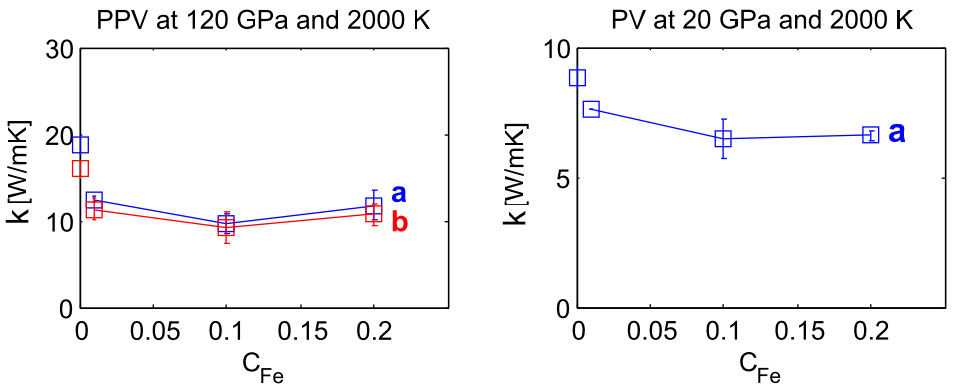
\includegraphics[width=\linewidth]{Figures/ammann_saturation.png}
  \caption[Thermal conductivity against Fe-content]{Thermal conductivity decrease due to inclusion of impurities is shown to saturate with increasing Fe-content, for \mgsios \ppv and perovskite phases. \textbf{a} and \textbf{b} refer to crystallographic directions along which conductivity was calculated. Figure modified from \citet{Ammann2014}.}
  \label{fig:ammann_sat}
\end{figure}

\citet{Tang2014} performed first-principles calculations to assess the \tcs of \mgsios
and the effect of Fe inclusions therein. These results feed into a model of conductivity along a lower mantle geotherm, of aggregate composition 4 \bdg : 1 periclase with 12.5\% Fe impurities. Their calculations model \mgfesios by increasing atomic mass, but not changing the force constants, in a manner similar to \citet{Ammann2014}. The inclusion of impurities has little effect at 136~GPa-4000~K, on the order of a few percent, but they note MgO is affected more considering its higher conductivity. The observation that conductivity is reduced less when it is already small due to the effect of temperature, matches the saturation described in \citet{Ammann2014}, but in turn disagrees with \citet{Haigis2012}. The uncertainity is large when experimental data is extrapolated, especially when considering the (temperature-dependent) effect of impurities.

%-------------------
\subsubsection{Radiative conductivity}
%-------------------
\label{sec:rad_cond}

\citet{Hofmeister1999} produced a model of thermal conductivity for the entire mantle using data from infrared reflectivity methods. The radiative component at maximum was found to be small compared to the lattice conductivity, between 10--15\% depending on the geotherm model used. This corresponds to radiative conductivity values of 0.67--0.82~\wmks compared to 5.8--6.7~\wmks for the total conductivity at the top of \ddd.

\citet{Keppler2008} studied the near-infrared and optical absorption spectra of silicate perovskite up to pressures of 125~GPa at room temperature. From both their tests and visual inspection, it can be shown that their synthesised perovskite remains transparent at high pressures. Extrapolating their results to high temperatures (4500~K) they suggest that the maximum radiative thermal conductivity above the CMB is around 10~\wmk, implying that radiative conductivity is likely to be an important component of the total conductivity at lower mantle conditions. The study does not measure the variation of absorption spectra with temperature and pressure, of which experimentation is currently unfeasible.

\citet{Goncharov2008} performed a similar optical absorption spectra analysis up to 133~GPa, but with the opposite conclusion to \citet{Keppler2008}. They agreed the radiative conductivity was dependent on the amount, redox state, and spin state of iron, but disagreed with its significance. \citet{Goncharov2008} estimated radiative conductivity would not exceed 0.54~\wmks at the top of the \ddds layer, a value in line with \citet{Hofmeister1999} and at odds with \citet{Keppler2008}. Until better constrained, it is convenient to assume the radiative component is small compared to the lattice component. As stated earlier (Section~\ref{sec:what_is_tc}), the two components can simply be added to determine the total thermal conductivity (for the lower mantle).

\citet{Tang2014} re-evaluated the works of \citet{Keppler2008} and \citet{Goncharov2008} to create a profile of radiative conductivity in the lower mantle. \citeauthor{Tang2014}'s profile suggests that the previous works have a more reasonable agreement than they show, using analysis which gives an upper bound on the conductivity. Radiative heat transfer is inhibited in the same way as conductive, by impurities and grain boundaries which are not considered when calculating this upper bound. Unlike lattice thermal conductivity, radiative conductivity increases with temperature, steeply so in the mantle thermal boundary layer. When the opposing temperature dependencies of lattice and radiative conductivity are considered in tandem, they suggest that the thermal conductivity of the lower mantle is largely temperature-independent above the \ddds region at around 3~\wmk. Thermal conductivity increases to 5.5 \wmks in the TBL, due to the increased significance of the radiative component.





%-----------------------------------------------------------
\section{Thesis outline}
%-----------------------------------------------------------
In Chapter \ref{Chapter2} we provide an overview of the methods and expand on issues. I outline my computational approaches, for the non-equilibrium molecular dynamics direct method and equilibrium molecular dynamics Green-Kubo method. I show convergence of computed conductivity with respect to simulation cell size and shape 

In Chapter \ref{Chapter3}, PRESSURE/TEMPERATURE EFFECTS. DISCUSS [P/T] SCALING LAW / THEORETICAL MODEL

In Chapter \ref{Chapter4}, ADAPTING SYSTEM TO INCLUDE IRON, DETERMINING EFFECT OF IMPURITY CONTENT, PRODUCING A MODEL OF THE LOWER MANTLE CONDUCTIVITY WITH VARIABLE TEMPERATURE AND BRIDGMANITE COMPOSITION

%---------------------------------------
\subsection{Aims}
%---------------------------------------

%---------------------------------------
\subsection{Objectives}
%---------------------------------------


